%Dokumententyp
\documentclass[a4paper]{article}

\usepackage[a4paper,left=2cm, right=3cm, top=2cm]{geometry}

%Kodierung
\usepackage[utf8]{inputenc}
\usepackage[T1]{fontenc}

%Grafiken einbinden
\usepackage{graphicx}
\usepackage{subfigure} 

%Position von Grafiken und Tabellen erzwingen:
\usepackage{float}

%URLs im Literaturverzeichnis
\usepackage{url}

\usepackage{amsmath}

%Vektoren einfacher angeben:
\newcommand{\vektor}[1]{\left( \begin{array}{c} #1 \end{array} \right) }


%Schriftart Arial:
% \usepackage{helvet}

%Figures with text around it:
\usepackage{wrapfig}

\usepackage{listings}

%seitennummern rechts:
% \usepackage{fancyhdr}
% \fancyhf{} % clear all header and footers
% \renewcommand{\headrulewidth}{0pt} % remove the header rule
% \rfoot{\thepage}
% \fancypagestyle{plain}{%redefining plain pagestyle
% \fancyhf %clear all headers and footers fields
% \fancyhead[R]{\thepage} %prints the page number on the right side of the header
% }

%Schriftart Times New Roman "like"
\usepackage{txfonts}

%Sprache
\usepackage[german]{babel}

%Checkmarks: (usage: \checkmark)
\usepackage{dingbat}

\usepackage{listings}
\usepackage{color}
\definecolor{javared}{rgb}{0.6,0,0} % for strings
\definecolor{javagreen}{rgb}{0.25,0.5,0.35} % comments
\definecolor{javapurple}{rgb}{0.5,0,0.35} % keywords
\definecolor{javadocblue}{rgb}{0.25,0.35,0.75} % javadoc
 
\lstset{language=Java,
basicstyle=\ttfamily,
keywordstyle=\color{javapurple}\bfseries,
stringstyle=\color{javared},
commentstyle=\color{javagreen},
morecomment=[s][\color{javadocblue}]{/**}{*/},
numbers=left,
numberstyle=\tiny\color{black},
stepnumber=1,
numbersep=5pt,
tabsize=4,
showspaces=false,
lineskip={-1.5pt},
showstringspaces=false}

%Tabellenextras
\usepackage{tabularx}

%Zeilenabstand 1.5
\linespread{1.5}
\usepackage{setspace}

%
\usepackage{cancel}

%Figure Captions mit Fußnoten
\usepackage{footnote}
%\setlength{\parindent}{0pt} 

%Graphen/Trees zeichnen:
\usepackage{tikz}
\newcommand*\circled[1]{\tikz[baseline=(char.base)]{
            \node[shape=circle,draw,inner sep=2pt] (char) {#1};}}


%itemize items richtig ausrichten (nicht links überlappen!)
% \setlist{leftmargin=0}

% %%%%TITELSEITE%%%%%%(
% \title{ Konzept und Implementierung\\ eines Systems zur \\Anforderung und Verwaltung von virtuellen privaten Clustern}
% \author{\textbf{\large Bachelorarbeit}}
% 
% \date{zur Erlangung des akademischen Grades Bachelor of Science an der Universität Paderborn im Fachbereich Informatik im Studiengang Bachelor Informatik}

% %%%%TITELSEITE%%%%%%)

% \pagestyle{fancy}
\begin{document}

\title{Algorithmische Geometrie - Sommersemester 2015\\
       9. Aufgabenblatt }
\author{Simon Koennecke und Felix Bröker}
\date{}
\maketitle

\section*{Aufgabe 1 - Platonische Körper}
\subsection*{(a)}
Um zu beweisen, dass es in 3 Dimensionen höchstens 5 platonische Körper gibt, 
greifen wir auf folgende Vorüberlegungen zurück:

\begin{itemize}
	\item Wir wissen: In jede Ecke eines 3-dimensionalen Polyeders "`münden"' mindestens 3 Kanten
	\item Entsprechend wissen wir: Damit dies auch im platonischen Körper gilt, muss jeweils 1 Ecke des Körpers
	mit je 1 Ecke von mindestens 3 zum Körper gehörenden regulären $m$-Ecken übereinstimmen. 
	\item Wir übertragen diese Forderung in den 2-dimensionalen Raum, welche analog lautet:
	Für jedes $m$-Eck eines platonischen Körpers muss gelten: Wir können mindestens 
	3 $m$-Ecke um eine zentrale, gemeinsame Ecke $z$ überlappungsfrei anordnen. Zudem muss außerdem gelten:
	Wenn wir die genannten $m$-Ecke außerdem mit ihren jeweiligen zur Ecke $z$ gehörenden Kanten
	verbinden, muss es 2 der $m$-Ecke geben, dessen Kanten, welche in $z$ münden 
	aufgrund der Distanz nicht miteinander verbunden, d.h. zur Deckung gebracht werden können.	
\end{itemize}

	\begin{figure}[!htb]
\subfigure[Beispiel von 3 überlappungsfreien 4-Ecken, dessen Kanten (z,i) nicht alle 
	"`verbunden"'/zur Deckung gebracht werden können]{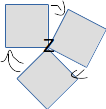
\includegraphics[width=0.25\textwidth]{aufgabe1a}} 
	\end{figure} 

Wir überlegen uns nun, für welche Werte von $m$ die genannte Forderung eingehalten 
werden kann. Dazu schauen wir uns an, wie groß der Innenwinkel einer Ecke 
eines $m$-Ecks ist. Für einfache n-Ecke gibt $(n-2)*180^{\circ}$ die Innenwinkelsumme an.
Da wir regelmäßige $m$-Ecke gegeben haben, ist die Größe eines Innenwinkels eines
regelmäßigen $m$-Ecks mit $\frac{(m-2)*180^{\circ}}{m}$ gegeben. Entsprechend gibt 
nun folgende Funktion an, wie viele $m$-Ecke wir maximal überlappungsfrei um eine zentrale Ecke $z$
im Kreis anordnen können: $f(m) = \frac{360^{\circ}}{\frac{(m-2)*180^{\circ}}{m}} = 
\frac{360^{\circ} * m}{(m-2) * 180^{\circ}} = \frac{2m}{m-2}$.

Wegen $f'(m) = -\frac{4}{(m-2)^2}$ ist $f(m \in (2,\infty))$ streng monoton fallend. 
Da wir in jedem Fall minimal 3 $m$-Ecke überlappungsfrei anordnen können müssen, 
setzen wir $f(m) = 3$ und erhalten $\frac{2m}{m-2} = 3 \Leftrightarrow m = 6$.
Das reguläre 6-Eck ist also das "`maximale"' $m$-Eck, bei dem wir gerade noch 3 
$m$-Ecke überlappungsfrei im Kreis um eine zentrale gemeinsame Ecke $z$ anordnen können.
Da wir jedoch wie beschrieben, zusätzlich jeweils eine Kante zweier $m$-Ecke
 mit Endpunkt in $z$ benötigen, welche aufgrund der Distanz nicht miteinander
 verbunden/zur Deckung gebracht werden können, muss gelten $f(m) > 3$.
 Das $m$-Eck mit $m = 6$ Ecken scheidet daher als Kandidat für einen platonischen Körper aus.
 Es verbleiben deshalb noch die "`Kandidaten"' $m = 3$, $m = 4$ und $m = 5$.
 Für $m = 5$ erhalten wir $f(5) = \frac{10}{3} = 3,\overline{3}$. Wir können also
 genau \textbf{3 5-Ecke} entsprechend um ein Zentrum $z$ anordnen und haben wegen des "`überlappenden"'
 Nachkommawertes von $0,\overline{3}$ entsprechende zwei Kanten die nicht mehr verbunden werden können.
 Für $m = 4$ sind entsprechend $f(4) = \frac{8}{2} = 4$ 4-Ecke um $z$ möglich, jedoch wieder ohne
 Nachkommastelle. Deshalb kann es nur noch den nächst niedrigeren Wert von \textbf{3 4-Ecken} geben.
 Für $m = 3$ erhalten wir $f(3) = \frac{6}{1} = 6$. Wegen der fehlenden Nachkommastelle, 
 erhalten wir wieder nur die nächst niedrigeren möglichen Werte von \textbf{5, 4 und 3 für m = 3}. 
 
 Insgesamt gibt es also höchstens die folgenden 5 Möglichkeiten eines platonischen Körpers:
 
 \begin{itemize}
 	\item 3 5-Ecke bilden eine Ecke  (existiert und wird "`Dodekaeder"' genannt)
 	\item 3 4-Ecke bilden eine Ecke  (existiert und wird "`Hexaeder"' genannt)
 	\item 5 3-Ecke bilden eine Ecke  (existiert und wird "`Ikosaeder"' genannt)
 	\item 4 3-Ecke bilden eine Ecke  (existiert und wird "`Oktaeder"' genannt)
 	\item 3 3-Ecke bilden eine Ecke  (existiert und wird "`Tetraeder"' genannt)
 \end{itemize}
 
 Wie wir in der Literatur nachschlagen können, sehen wir, dass diese Möglichkeiten 
 in Form der aufgeführten Bezeichnungen auch wirklich existieren.
  

\subsection*{(b)}
\begin{figure}[!htb]
\subfigure[Geometrischer Graph (d.h. planarer Graph) des Ikosaeders]{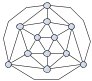
\includegraphics[width=0.25\textwidth]{ikosaeder}} 
\subfigure[Geometrischer Graph (d.h. planarer Graph) des Dodekaeders]{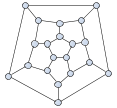
\includegraphics[width=0.25\textwidth]{dodekaeder}} 
\end{figure} 

\section*{Aufgabe 2 - d-dimensionale Polytope}

\subsection*{(a)}
Die Ecken $W_{c(d)}$ eines d-dimensionalen Einheitswürfels $W_d$ sind gegeben mit

$W_{c(d)}=\{(x_1, ..., x_d) \in \mathcal{R}^d : x_1, ..., x_d \in \{0, 1\}\}$, 
wobei gilt $|W_{c(d)}| = 2^d$.

Sei $I \in \mathcal{R}^{d x d}$ die $d$-dimensionale Einheitsmatrix, 
$\vec{0}_d$ der d-dimensionale 0-Vektor und $\vec{1}_d$ der d-dimensionale
1-Vektor.

Dann sind die $d-1$-dimensionalen Facetten $W_{f_{d-1}(d)}$ von $W_d$ gegeben mit:

$W_{f_{d-1}(d)} = \{\vec{0}_d + x_1 e_{i1} + ... + x_{d-1} e_{i(d-1)}\} \cup \{\vec{1}_d - x_1 e_{i1} - ... - x_{d-1} e_{i(d-1)}\}$, wobei $x_i \in [0,1]$ und $e_{ij}$ Spaltenvektor von $I$.
Zudem muss für ein beliebiges aber festes $i$ gelten, dass die Vektoren $e_{ij}$ paarweise
verschieden sind. Und es muss für ein beliebiges aber festes $i_a$ 
und ein beliebiges aber festes $i_b$ mit $i_a \neq i_b$ gelten: 
$\{e_{i_1j}\} \neq \{e_{i_2j}\}$ (Es sollen alle Kombinationen von Einheitsvektoren in den Gleichungen berücksichtigt werden).

Für die Größe von $W_{f_{d-1}(d)}$ gilt $|W_{f_{d-1}(d)}| = 2*d$.

\subsection*{(b)}
\begin{figure}[!htb]
\subfigure[Skizze eines $W_4$ Hypercubes]{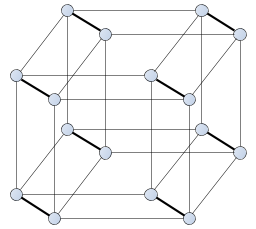
\includegraphics[width=0.25\textwidth]{hypercube}} 
\end{figure} 

\subsection*{(c)}

\begin{figure}[!htb]
\subfigure[Skizze eines $S_4$ Hypertetraeders]{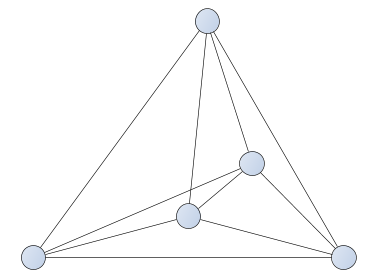
\includegraphics[width=0.25\textwidth]{hypertetraeder}} 
\end{figure} 

Wie in Aufgabe a greifen wir im Folgenden wieder auf die Einheitsmatrix $I$ und deren Einheitsvektoren $\vec{e_i}$ etc. zurück.
Die $d-1$-dimensionalen Facetten $S_{f_{d-1}(d)}$ von $S_d$ sind gegeben mit:

$\{\vec{0_d} + x_1\vec{e_{i_1}} +  x_2\vec{e_{i_2}} + \dots  + x_{d-1}\vec{e_{i_{d-1}}} | \sum_{i=1}^{d-1}x_i \leq 1\} \cup 
\{\vec{e_1} + x_1  (\vec{e_2}-\vec{e_1}) + x_2(\vec{e_3}-\vec{e_1}) + \dots + x_{d-1}(\vec{e_{d-1}} - \vec{e_1}) |  \sum_{i=1}^{d-1} x_i \leq 1 \}$

Zudem muss für ein beliebiges aber festes $i$ gelten, dass die Vektoren $e_{ij}$ paarweise
verschieden sind. Und es muss für ein beliebiges aber festes $i_a$ 
und ein beliebiges aber festes $i_b$ mit $i_a \neq i_b$ gelten: 
$\{e_{i_aj}\} \neq \{e_{i_bj}\}$ (Es sollen alle Kombinationen von Einheitsvektoren in den Gleichungen berücksichtigt werden).

Für die Größe von $S_{f_{d-1}(d)}$ gilt $|S_{f_{d-1}(d)}| = d+1$.


\section*{Aufgabe 3 - Konvexe Hülle}
Sei die Punktmenge $S \subset \mathcal{R}^3$ gegeben mit $|S| = n$.
Zur Vereinfachung nehmen wir an, dass die Punkte aus $S$ in allgemeiner Lage sind.
Die konvexe Hülle $CH(S)$ kann daher auch als eine Menge von Facetten $F$, welche Dreiecke sind, 
aufgefasst werden.

Da je 3 Punkte $\in S$ eine Ebene definieren und wir wissen, dass für alle Flächen $\in F$ 
gelten muss, dass alle anderen Punkte $\in S$ nur in einem durch diese Fläche/Ebene definierten Halbraum
liegen dürfen, haben wir uns folgenden einfachen Brute-Force-Algorithmus überlegt:

\textbf{
\begin{itemize}
	\item Für alle "`3-Punkte-Kombinationen"' $(p_i, p_j, p_k)$ von Punkten $\in S$:
	\begin{itemize}
		\item Prüfe, ob jeweils alle anderen Punkte $\{p | p \in S \wedge p \neq p_i, p_j, p_k\}$ 
		nur in einem der Halbräume der durch $(p_i, p_j, p_k)$ definierten Ebene liegen.	
		\item Falls ja, füge die Facette $f$ mit den Eckpunkten $p_i, p_j, p_k$ zu $F$ hinzu.
	\end{itemize}
\end{itemize}
}

Es werden also ganz im Sinne von Brute-Force stumpf alle möglichen 3er-Kombinationen von Punkten
durchgetestet und nur die als Facette zur Lösung $F$ hinzugefügt, welche die Eigenschaft einer
zur konvexen Hülle $CH(S)$ gehörenden Facette erfüllen. 

\subsubsection*{Laufzeit}
Die Laufzeit des Brute-Force-Algorithmus lässt sich relativ einfach wie folgt abschätzen:
\begin{itemize}
	\item Es gibt genau  $\binom{n}{3}$  "`3-Punkte-Kombinationen"'. Der beschriebene Schleifenrumpf
	wird daher genau $\binom{n}{3}$ mal ausgeführt.
	\item Das Prüfen, ob alle anderen Punkte nur in einem der Halbräume liegen, kann mit 
	$\mathcal{O}(n)$ abgeschätzt werden, denn die Prüfung für einen Punkt benötigt bekanntermaßen
	konstante Zeit. Dies muss entsprechend für $n-3 = \mathcal{O}(n)$ Punkte wiederholt werden.
	\item Falls die Prüfung positiv verläuft, kann die entsprechende Facette $f$ in konstanter Zeit
	in $F$ eingefügt werden (in einer konkreten Implementation z.B. durch Anhängen von $f$ 
	an eine Liste $F$).
\end{itemize}

Damit ergibt sich eine Gesamtlaufzeit von:

\begin{align*}
\binom{n}{3} * (\underbrace{\mathcal{O}(n) + \mathcal{O}(1))}_{= \mathcal{O}(n)} &= 
\frac{n!}{3! * (n-3)!} * \mathcal{O}(n) \\
&= \frac{n * (n-1) * (n-2) * \cancel{(n-3) * \dots * 1}}{6 * \cancel{(n-3)!}} * \mathcal{O}(n) \\
&= \frac{n^3 - 3n^2 + 2n}{6} * \mathcal{O}(n) \\
&= \mathcal{O}(n^3) * \mathcal{O}(n) \\&= \mathcal{O}(n^4)
\end{align*}

\subsubsection*{Speicherplatzbedarf}
Beim Hinzufügen der Punkte werden nur Dreiecke als Facetten aufgenommen (Da die Punkte in allgemeiner Lage sind können die Facetten nur Dreiecke sein.). Daher hat jede Facette 3 Ecken und wir wissen, dass jeder Punkt aus der Menge $S$ linear viele Facetten nach der Eulerformel (Dualität planarer Graph) hat. Daraus resultiert der Speicherplatzbedarf von $\mathcal{O}(n)$


\end{document}

